\documentclass{amsart}

\usepackage{amsmath,amssymb,amsthm}
\usepackage[hidelinks]{hyperref}
\usepackage[noabbrev,capitalize]{cleveref}
\usepackage{graphicx}
\usepackage{enumitem}
\usepackage{booktabs}
\usepackage{algorithm}
\usepackage[noend]{algpseudocode}

% Theorem environments
\newtheorem{theorem}{Theorem}[section]
\newtheorem{lemma}[theorem]{Lemma}
\newtheorem{proposition}[theorem]{Proposition}
\newtheorem{corollary}[theorem]{Corollary}
\newtheorem{conjecture}[theorem]{Conjecture}

\theoremstyle{definition}
\newtheorem{definition}[theorem]{Definition}
\newtheorem{example}[theorem]{Example}
\newtheorem{assumption}[theorem]{Assumption}

\theoremstyle{remark}
\newtheorem{remark}[theorem]{Remark}

\numberwithin{equation}{section}

% Import command files (if they exist)
\InputIfFileExists{commands/math}{}{}
\InputIfFileExists{commands/general}{}{}
\InputIfFileExists{commands/macros}{}{}

% Project-specific shorthands
\newcommand{\RC}{\mathrm{RC}}
\newcommand{\clip}{\mathrm{clip}}
\renewcommand{\eth}{\mathrm{eth}}
\newcommand{\acc}{\mathrm{acc}}
\newcommand{\rob}{\mathrm{rob}}
\newcommand{\nat}{\mathrm{nat}}

\title[Quantifying Ethical Robustness in Adversarial ML Systems]{A Composite Coefficient for Quantifying Ethical Robustness in Adversarial Machine-Learning Systems}

\author{NeuriCo}
\email{chicagohailab@gmail.com}

\subjclass[2020]{Primary 68T05, 68T27; Secondary 90C40, 62P99}

\date{July 2, 2026}

\keywords{Adversarial robustness, certified robustness, alignment, constrained
Markov decision processes, composite metrics, robustness--accuracy trade-off}

\begin{document}

\begin{abstract}
Machine-learning systems deployed in scientific and high-stakes settings are
routinely certified by a single scalar---accuracy---that is provably blind to the
ethical failure modes (bias, integrity, transparency collapse) that adversarial
prompts can induce while correctness is preserved. We formalize the informal
hypothesis that models trained under explicit ethical constraints are more robust
under adversarial perturbation, and that this gain is captured by a composite
metric. We introduce the \emph{composite ethical-robustness coefficient}
$\RC_\lambda(f,x,\varepsilon)=\lambda\,\rho_C+(1-\lambda)\,\rho_A$, a convex
combination of the worst-case preservation ratios of scientific correctness and
ethical alignment over an adversarial perturbation set, and prove six results
about it. We show that $\RC_\lambda$ is well-posed (bounded in $[0,1]$, monotone
non-increasing in the perturbation radius, exact at radius zero); that its deficit
admits an exact TRADES-style additive decomposition into correctness- and
alignment-stability terms; and---our central result---that a training-time
constrained-Markov-decision-process alignment constraint, together with a bounded
correctness cost, forces a provable separation between the constrained and the
accuracy-only model that exceeds the target $0.15$ on an explicit, checkable
parameter region. We further prove that the composite is \emph{necessary}: every
correctness-only metric is provably blind to alignment collapse, whereas
$\RC_\lambda$ separates a safe from a collapsed model by $1-\lambda$. Finally, we
give attack-independent Lipschitz and randomized-smoothing certified lower bounds.
Every algebraic step is machine-checked with a computer-algebra system, and every
quantitative claim with a seeded Monte-Carlo study.

\end{abstract}

\maketitle

\section{Introduction}
\label{sec:intro}

\subsection{Motivation}
Machine-learning systems in scientific and safety-critical domains are almost
universally judged by a single scalar: accuracy, or one of its robust variants.
This is convenient, but it is also mathematically incomplete. A model may answer a
scientific question correctly and yet, under an adversarially crafted prompt,
silently violate the ethical requirements we care about---fabricating citations,
amplifying bias, leaking private information, or abandoning transparency---while
its answer remains nominally right. An accuracy-only report certifies such a model
as safe. The gap is not a matter of measurement noise: it is structural. A metric
that depends on the model only through its correctness behavior \emph{cannot}, as a
matter of logic, detect a failure that leaves correctness untouched.

This motivates a precise mathematical question. Adversarial-robustness theory has
produced rigorous, quantitative coefficients for the stability of
\emph{correctness} under perturbation---the CLEVER score built from local Lipschitz
constants \cite{Weng2018}, the certified radius of randomized smoothing
\cite{Cohen2019}, and the exact robust-error decomposition of TRADES
\cite{Zhang2019}. Alignment research has, in parallel, produced quantitative
measures of \emph{ethical} stability, chiefly the attack success rate against
standardized jailbreak benchmarks \cite{Chao2024,Zou2023}. These two literatures
have not been fused: to our knowledge no prior work combines a
certified-robustness-style correctness term with an alignment-stability term into a
single coefficient with provable properties, and none connects a training-time
ethical constraint to a lower bound on such a coefficient.

\subsection{The question}
We study the following informal hypothesis, which arises repeatedly in the
empirical literature on aligned models: \emph{models trained with explicit ethical
constraints are at least $0.15$ more robust than accuracy-only models under
adversarial prompts, and this improvement is captured by a composite metric.} We
ask whether this can be turned into a theorem. Concretely: is there a precisely
defined coefficient $\RC_\lambda$ with provable analytic properties, together with
explicit sufficient conditions under which a training-time ethical constraint
\emph{guarantees} a separation
\[
  \Delta \;=\; \E[\RC_\lambda^{\eth}] - \E[\RC_\lambda^{\acc}] \;\ge\; 0.15\,?
\]
And is such a composite \emph{necessary}, or does accuracy alone already suffice?

\subsection{Contributions}
We answer both questions affirmatively. We define the composite ethical-robustness
coefficient
\[
  \RC_\lambda(f,x,\varepsilon) \;=\; \lambda\,\rho_C(f,x,\varepsilon)
    + (1-\lambda)\,\rho_A(f,x,\varepsilon), \qquad \lambda\in[0,1],
\]
where $\rho_C,\rho_A\in[0,1]$ are the worst-case preservation ratios of scientific
correctness $C$ and ethical alignment $A$ over an adversarial perturbation set
$B(x,\varepsilon)$, and prove:

\begin{itemize}[leftmargin=*,itemsep=2pt,topsep=2pt]
  \item \textbf{Well-posedness (\Cref{thm:wellposed}).} $\RC_\lambda$ is bounded in
  $[0,1]$, non-increasing in $\varepsilon$, equal to $1$ at $\varepsilon=0$, and
  recovers the single-term correctness and alignment metrics at $\lambda=1$ and
  $\lambda=0$.
  \item \textbf{Exact decomposition (\Cref{thm:decomp}).} The deficit of each
  component obeys an exact additive identity $e_\rob^S=e_\nat^S+b^S$, the direct
  analogue of the TRADES identity $R_\rob=R_\nat+R_\mathrm{bdy}$ \cite{Zhang2019},
  yielding a normalized upper bound on $1-\E[\RC_\lambda]$.
  \item \textbf{Constraint $\Rightarrow$ separation (\Cref{thm:main}, central).} A
  constrained-Markov-decision-process alignment constraint on the ethical model,
  together with a bounded correctness cost $\delta_C$, forces
  $\Delta \ge (1-\lambda)\big[(1-d)-\bar a/a_{\min}\big]-\lambda\delta_C$, which
  meets the $0.15$ target on an explicit region.
  \item \textbf{Necessity of the composite (\Cref{thm:necessity}).} There exist two
  models indistinguishable to every correctness-only metric yet separated by
  $\RC_\lambda$; hence $\lambda<1$ is necessary to detect alignment collapse and
  $\lambda>0$ to detect correctness collapse.
  \item \textbf{Certified lower bounds (\Cref{thm:certified}).} $\RC_\lambda$
  admits attack-independent Lipschitz and randomized-smoothing certified lower
  bounds.
  \item \textbf{Admissible-weight region (\Cref{thm:lambda}).} The set of weights
  $\lambda$ achieving any target separation is characterized in closed form.
\end{itemize}

Although the correctness score $C$ is specialized in our motivating application to
correctness on astrophysics questions, every theorem below is stated for arbitrary
measurable scores $C,A\in[0,1]$ and is therefore domain-agnostic.

\subsection{Techniques}
The proofs are elementary but structured. Well-posedness and the decomposition
follow from the nesting property of perturbation sets and linearity of
expectation. The central separation theorem imports constrained-Markov-decision-
process feasibility \cite{Achiam2017} as the mechanism that turns an ethical
\emph{training constraint} into an alignment-robustness \emph{floor}, and combines
it with a clean-competence floor via two elementary bounds on the preservation
ratio. Necessity is proved by an explicit two-model hard-instance construction in
the style of \cite{Tsipras2018}. The certified bounds instantiate the Lipschitz
margin argument of \cite{Weng2018} and the Neyman--Pearson certificate of
\cite{Cohen2019}. Every symbolic identity and inequality is verified with a
computer-algebra system, and every quantitative claim is checked by a seeded
Monte-Carlo study; \Cref{sec:discussion} reports these.

\subsection{Organization}
\Cref{sec:prelim} fixes notation, states the definitions, and recalls the
prerequisite results. \Cref{sec:results} states and proves the six theorems, with
worked examples. \Cref{sec:discussion} reports the computational verification and
discusses implications, limitations, and open problems. \Cref{sec:conclusion}
concludes.

\section{Preliminaries}
\label{sec:prelim}

\subsection{Notation}
Inputs $x$ are drawn from a distribution $D$ on an input space $\mathcal{X}$, and
$f$ denotes a fixed model. Expectations $\E[\cdot]$ are over $x\sim D$ unless
otherwise indicated. We write $\Phi$ for the standard-normal cumulative
distribution function and $\Phi^{-1}$ for its inverse. For $a\le b$ and a real
number $t$ we write $\clip(t,a,b)=\min\{\max\{t,a\},b\}$.

\subsection{Perturbation sets}
An adversary is modeled by a family of \emph{perturbation sets}
$\{B(x,\varepsilon)\}_{\varepsilon\ge0}$, one per input, indexed by a radius
$\varepsilon\ge0$. We require two structural axioms.

\begin{definition}[Admissible perturbation family]\label{def:pert}
A family $\{B(x,\varepsilon)\}$ is \emph{admissible} if it satisfies
\begin{enumerate}[label=\textup{(P\arabic*)},leftmargin=*]
  \setcounter{enumi}{-1}
  \item \label{P0} $B(x,0)=\{x\}$ for every $x$;
  \item \label{P1} \emph{(nesting)} $\varepsilon_1\le\varepsilon_2$ implies
  $B(x,\varepsilon_1)\subseteq B(x,\varepsilon_2)$.
\end{enumerate}
\end{definition}

Both axioms hold for $\ell_p$ balls $B_p(x,\varepsilon)=\{x':\|x'-x\|_p\le
\varepsilon\}$ and, in the prompt setting, for families of adversarial prompts
measured by suffix length, edit distance, or token-substitution radius; this is the
sense in which our results specialize to the discrete adversarial-prompt threat
models of \cite{Zou2023,Chao2024}.

\subsection{Scores and preservation ratios}
The model is scored on two axes.

\begin{definition}[Scores and worst-case scores]\label{def:scores}
Let $C(f,x)\in[0,1]$ and $A(f,x)\in[0,1]$ be the clean \emph{scientific-correctness}
and \emph{ethical-alignment} scores at $x$; the alignment score aggregates
dimensions such as bias, reproducibility, transparency, integrity, and privacy, and
is of the form $A=1-\mathrm{ASR}$ in the sense of \cite{Chao2024}. The
\emph{worst-case scores} over $B(x,\varepsilon)$ are
\[
  \bar C(f,x,\varepsilon)=\min_{x'\in B(x,\varepsilon)}C(f,x'),
  \qquad
  \bar A(f,x,\varepsilon)=\min_{x'\in B(x,\varepsilon)}A(f,x').
\]
\end{definition}

By \ref{P0} and \ref{P1}, $\bar C\le C$, $\bar A\le A$ pointwise, with equality at
$\varepsilon=0$.

\begin{definition}[Component robustness and composite coefficient]\label{def:rc}
Fix a floor $\tau\in(0,1)$. The \emph{component robustness ratios} are
\[
  \rho_C(f,x,\varepsilon)=\clip\!\Big(\tfrac{\bar C(f,x,\varepsilon)}{\max(C(f,x),\tau)},0,1\Big),
  \qquad
  \rho_A(f,x,\varepsilon)=\clip\!\Big(\tfrac{\bar A(f,x,\varepsilon)}{\max(A(f,x),\tau)},0,1\Big).
\]
For a weight $\lambda\in[0,1]$, the \emph{composite ethical-robustness coefficient}
is
\[
  \RC_\lambda(f,x,\varepsilon)=\lambda\,\rho_C(f,x,\varepsilon)+(1-\lambda)\,\rho_A(f,x,\varepsilon),
\]
and its population version is $\RC_\lambda(f,\varepsilon)=\E_x[\RC_\lambda(f,x,\varepsilon)]$.
\end{definition}

The floor $\tau$ guards against division by a vanishing clean score; it is active
only on the event $\{C<\tau\}$ or $\{A<\tau\}$, and the outer $\clip$ ensures
$\rho_C,\rho_A\in[0,1]$ regardless.

\begin{definition}[Deficit quantities]\label{def:deficit}
For a score $S\in\{C,A\}$ write the \emph{natural deficit}
$e_\nat^S=\E[1-S]$, the \emph{robust deficit} $e_\rob^S=\E[1-\bar S]$, and the
\emph{stability gap} $b^S=\E[S-\bar S]\ge0$.
\end{definition}

\subsection{Regularity and constraint hypotheses}
Several results use clean-competence floors and Lipschitz regularity.

\begin{definition}[Clean floors and Lipschitz constants]\label{def:reg}
We say the model has \emph{clean floors} $c_{\min},a_{\min}\in(0,1]$ if
$C(f,x)\ge c_{\min}$ and $A(f,x)\ge a_{\min}$ almost surely. We say $C(f,\cdot)$ is
$L_C$-Lipschitz on $B(x,\varepsilon)$ if $|C(f,x')-C(f,x'')|\le L_C\,d(x',x'')$ for
all $x',x''\in B(x,\varepsilon)$, and similarly $L_A$ for $A(f,\cdot)$, where
$d(\cdot,\cdot)$ is the metric defining the perturbation set.
\end{definition}

The mechanism connecting ethical training to robustness is modeled after the
constrained-Markov-decision-process (CMDP) feasibility that constrained policy
optimization enforces \cite{Achiam2017}. Concretely, we distinguish two training
regimes through their alignment behavior under the adversary.

\begin{definition}[Constraint and collapse models]\label{def:ec}
The \emph{ethically constrained} model $f_\eth$ satisfies the alignment constraint
\begin{equation}\label{eq:EC}
  \E[\,1-\bar A(f_\eth,\cdot,\varepsilon)\,]\le d \tag{EC}
\end{equation}
for a tolerance $d\in[0,1)$, equivalently $\E[\bar A_\eth]\ge 1-d$. The
\emph{accuracy-only} model $f_\acc$ may collapse under the adversary:
\begin{equation}\label{eq:CO}
  \E[\,\bar A(f_\acc,\cdot,\varepsilon)\,]\le \bar a \tag{CO}
\end{equation}
for a collapse level $\bar a\in[0,1]$.
\end{definition}

Constraint \eqref{eq:EC} is exactly the CMDP feasibility $J_C(\pi_\eth)\le d$ of
\cite[Def.~2, Prop.~2]{Achiam2017}, realizable in practice by the constitution of
Constitutional AI \cite{Bai2022a} or the KL-regularized reward of RLHF
\cite{Ouyang2022,Bai2022b}; the collapse \eqref{eq:CO} models the empirically
documented jailbreak vulnerability of unconstrained models \cite{Zou2023}.

\subsection{Prerequisite results}
We use, without reproof, the following classical statements.

\begin{theorem}[TRADES decomposition {\cite[Def.~2.1--2.3]{Zhang2019}}]\label{thm:trades}
For a binary classifier the robust error decomposes exactly as
$R_\rob(f)=R_\nat(f)+R_\mathrm{bdy}(f)$, a clean-error term plus a non-negative
boundary term.
\end{theorem}

\begin{theorem}[Certified radius {\cite[Thm.~1]{Cohen2019}}]\label{thm:cohen}
Let $g$ be the Gaussian smoothing of a base classifier with variance $\sigma^2$. If
at $x$ the top and runner-up class probabilities under the smoothing noise satisfy
$p_A\ge p_B$, then $g$ is constant on the $\ell_2$-ball of radius
$R=\tfrac{\sigma}{2}\big(\Phi^{-1}(p_A)-\Phi^{-1}(p_B)\big)$ about $x$.
\end{theorem}

\begin{theorem}[Lipschitz margin bound {\cite[Cor.~2.1]{Weng2018}}]\label{thm:clever}
If the class-margin function of a classifier is $L$-Lipschitz on $B_p(x,R)$, then
the minimum distortion required to change its prediction at $x$ is at least the
margin at $x$ divided by $L$.
\end{theorem}

\section{Main Results}
\label{sec:results}

Throughout, \ref{P0} and \ref{P1} give $\bar C\le C$ and $\bar A\le A$ pointwise;
the floor $\tau$ matters only on the event $\{C<\tau\}$ or $\{A<\tau\}$, which is
handled uniformly by the outer $\clip$.

\subsection{Well-posedness}

\begin{theorem}[Well-posedness]\label{thm:wellposed}
For all $\lambda\in[0,1]$, $\varepsilon\ge0$, and $x$:
\begin{enumerate}[label=\textup{(\alph*)},leftmargin=*]
  \item $\RC_\lambda(f,x,\varepsilon)\in[0,1]$;
  \item under \ref{P1}, $\varepsilon\mapsto\RC_\lambda(f,x,\varepsilon)$ is
  non-increasing;
  \item under \ref{P0}, if $C(f,x),A(f,x)\ge\tau$ then
  $\RC_\lambda(f,x,0)=1$;
  \item $\RC_\lambda$ is affine and non-decreasing in each of $\rho_C,\rho_A$, with
  $\RC_1=\rho_C$ and $\RC_0=\rho_A$.
\end{enumerate}
\end{theorem}

\begin{proof}
\emph{(a)} By construction $\rho_C,\rho_A\in[0,1]$, since both are clipped to
$[0,1]$. For $\lambda\in[0,1]$ the quantity $\RC_\lambda=\lambda\rho_C+(1-\lambda)
\rho_A$ is a convex combination of two numbers in $[0,1]$: hence
$\RC_\lambda\ge\lambda\cdot0+(1-\lambda)\cdot0=0$ and
$\RC_\lambda\le\lambda\cdot1+(1-\lambda)\cdot1=1$.

\emph{(b)} Let $\varepsilon_1\le\varepsilon_2$. By \ref{P1},
$B(x,\varepsilon_1)\subseteq B(x,\varepsilon_2)$, so the minimum over the larger set
is no larger:
$\bar C(f,x,\varepsilon_2)=\min_{B(x,\varepsilon_2)}C
\le\min_{B(x,\varepsilon_1)}C=\bar C(f,x,\varepsilon_1)$. Dividing by the
$\varepsilon$-independent positive quantity $\max(C,\tau)$ and applying the
non-decreasing map $\clip(\cdot,0,1)$ preserves the inequality, so
$\rho_C(f,x,\varepsilon_2)\le\rho_C(f,x,\varepsilon_1)$; identically for $\rho_A$. A
non-negatively weighted sum of non-increasing functions is non-increasing, whence
the claim.

\emph{(c)} By \ref{P0}, $B(x,0)=\{x\}$, so $\bar C(f,x,0)=C(f,x)$ and
$\bar A(f,x,0)=A(f,x)$. If $C,A\ge\tau$ then $\max(C,\tau)=C$ and $\max(A,\tau)=A$,
so $\rho_C=C/C=1$ and $\rho_A=A/A=1$; hence
$\RC_\lambda(f,x,0)=\lambda+(1-\lambda)=1$.

\emph{(d)} As a function of the pair $(\rho_C,\rho_A)$ the map is affine with
partial derivatives $\partial\RC_\lambda/\partial\rho_C=\lambda\ge0$ and
$\partial\RC_\lambda/\partial\rho_A=1-\lambda\ge0$, hence non-decreasing in each.
Substituting $\lambda=1$ gives $\RC_1=\rho_C$ (the correctness-only robustness
metric of \cref{thm:clever,thm:cohen}) and $\lambda=0$ gives $\RC_0=\rho_A$ (the
alignment-only, $1-\mathrm{ASR}$ metric of \cite{Chao2024}).
\end{proof}

Part~(d) shows that the two established single-axis metrics are the endpoints of a
one-parameter family; every interior $\lambda$ is a genuine composite. The
following example records the intended reading of $\RC_\lambda$.

\begin{example}\label{ex:reading}
Suppose a model is perfectly correct-robust, $\rho_C=1$, but loses half its
alignment margin under attack, $\rho_A=\tfrac12$. Then
$\RC_{1}=1$ reports no problem, $\RC_{0}=\tfrac12$ reports the full problem, and
$\RC_{1/2}=\tfrac34$ reports a proportionate blend. Only $\lambda<1$ registers the
alignment loss at all; \cref{thm:necessity} makes this dichotomy exact.
\end{example}

\subsection{Exact decomposition}

\begin{theorem}[Exact decomposition and normalized bound]\label{thm:decomp}
For each score $S\in\{C,A\}$ the identity
\begin{equation}\label{eq:decomp}
  e_\rob^S=e_\nat^S+b^S
\end{equation}
holds exactly. Consequently, if the model has clean floors $c_{\min},a_{\min}$
\textup{(\cref{def:reg})}, then
\begin{equation}\label{eq:normbound}
  1-\E[\RC_\lambda]
    =\lambda\,\E\!\Big[\tfrac{C-\bar C}{C}\Big]
     +(1-\lambda)\,\E\!\Big[\tfrac{A-\bar A}{A}\Big]
    \le \lambda\,\frac{b^C}{c_{\min}}+(1-\lambda)\,\frac{b^A}{a_{\min}}.
\end{equation}
\end{theorem}

\begin{proof}
\emph{Decomposition.} Fix $S\in\{C,A\}$ and any $x$. Since $\bar S\le S$, the
identity $1-\bar S=(1-S)+(S-\bar S)$ holds pointwise, with $S-\bar S\ge0$. Taking
$\E_{x\sim D}$ and using linearity of expectation gives
$e_\rob^S=\E[1-\bar S]=\E[1-S]+\E[S-\bar S]=e_\nat^S+b^S$. This is the exact
analogue of the TRADES identity of \cref{thm:trades}: a clean term plus a
non-negative stability term.

\emph{Normalized bound.} Suppose $C\ge c_{\min}>0$ almost surely. Then $\tau$ is
inactive and $0\le\bar C\le C$, so the inner clip in $\rho_C$ is inactive and
$\rho_C=\bar C/C$, whence $1-\rho_C=(C-\bar C)/C$. Because $0<c_{\min}\le C$ and
$C-\bar C\ge0$, we have $(C-\bar C)/C\le(C-\bar C)/c_{\min}$; taking expectations,
$\E[1-\rho_C]\le\E[C-\bar C]/c_{\min}=b^C/c_{\min}$, and symmetrically
$\E[1-\rho_A]\le b^A/a_{\min}$. Finally, by linearity,
\[
  1-\E[\RC_\lambda]=\E\big[\lambda(1-\rho_C)+(1-\lambda)(1-\rho_A)\big]
    =\lambda\,\E[1-\rho_C]+(1-\lambda)\,\E[1-\rho_A],
\]
which gives the stated equality and, combining the two component bounds, the
inequality.
\end{proof}

\subsection{Constraint implies separation}

We now state the central result: an ethical training constraint provably separates
the constrained model from the accuracy-only one.

\begin{theorem}[Constraint $\Rightarrow$ separation]\label{thm:main}
Assume the alignment constraint \eqref{eq:EC} on $f_\eth$, the collapse
\eqref{eq:CO} on $f_\acc$, the clean floor $A(f_\acc,\cdot)\ge a_{\min}$ almost
surely, and a correctness-robustness cost bound
\begin{equation}\label{eq:costbound}
  \E[\rho_C^{\acc}]-\E[\rho_C^{\eth}]\le\delta_C.
\end{equation}
Then the separation $\Delta=\E[\RC_\lambda^{\eth}]-\E[\RC_\lambda^{\acc}]$ satisfies
\begin{equation}\label{eq:main}
  \Delta \;\ge\; (1-\lambda)\big[(1-d)-\bar a/a_{\min}\big]-\lambda\delta_C.
\end{equation}
In particular, whenever the right-hand side of \eqref{eq:main} is at least $0.15$,
the hypothesis' target $\Delta\ge0.15$ holds.
\end{theorem}

\begin{proof}
Write $\E[\RC_\lambda^m]=\lambda\E[\rho_C^m]+(1-\lambda)\E[\rho_A^m]$ for
$m\in\{\eth,\acc\}$, so that
\begin{equation}\label{eq:star}
  \Delta=\lambda\big(\E[\rho_C^{\eth}]-\E[\rho_C^{\acc}]\big)
        +(1-\lambda)\big(\E[\rho_A^{\eth}]-\E[\rho_A^{\acc}]\big).
\end{equation}

\emph{Step 1 (lower bound the ethical alignment term).} For every $x$ we have
$A(f_\eth,x)\le1$, hence $\max(A_\eth,\tau)\le1$ (as $\tau<1$) and
$\rho_A^{\eth}=\clip(\bar A_\eth/\max(A_\eth,\tau),0,1)\ge \bar A_\eth$, since
dividing by a number $\le1$ only increases the value and the clip to $[0,1]$ can
only raise a value below $1$. Taking expectations and applying \eqref{eq:EC},
\begin{equation}\label{eq:step1}
  \E[\rho_A^{\eth}]\ge\E[\bar A_\eth]\ge 1-d.
\end{equation}

\emph{Step 2 (upper bound the accuracy-only alignment term).} Since
$A_\acc\ge a_{\min}$ almost surely, $\tau$ is inactive and
$\rho_A^{\acc}=\clip(\bar A_\acc/A_\acc,0,1)\le \bar A_\acc/a_{\min}$, because
$A_\acc\ge a_{\min}$ makes the ratio at most $\bar A_\acc/a_{\min}$ and the clip can
only lower it. Taking expectations and applying \eqref{eq:CO},
\begin{equation}\label{eq:step2}
  \E[\rho_A^{\acc}]\le\E[\bar A_\acc]/a_{\min}\le \bar a/a_{\min}.
\end{equation}
Subtracting \eqref{eq:step2} from \eqref{eq:step1},
\begin{equation}\label{eq:step12}
  \E[\rho_A^{\eth}]-\E[\rho_A^{\acc}]\ge (1-d)-\bar a/a_{\min}=:\gamma_A.
\end{equation}

\emph{Step 3 (control the correctness term).} The cost bound
\eqref{eq:costbound} is exactly $\E[\rho_C^{\eth}]-\E[\rho_C^{\acc}]\ge-\delta_C$.

\emph{Step 4 (combine).} Substituting \eqref{eq:step12} and Step~3 into
\eqref{eq:star}, and using $\lambda\ge0$, $1-\lambda\ge0$ to combine the two
inequalities linearly,
\[
  \Delta\ge\lambda(-\delta_C)+(1-\lambda)\gamma_A
    =(1-\lambda)\big[(1-d)-\bar a/a_{\min}\big]-\lambda\delta_C,
\]
which is \eqref{eq:main}.
\end{proof}

\begin{corollary}[The $\ge0.15$ claim]\label{cor:015}
If $(1-\lambda)\big[(1-d)-\bar a/a_{\min}\big]-\lambda\delta_C\ge0.15$, then
$\Delta\ge0.15$. For the parameters
$\lambda=\tfrac12,\ d=\tfrac14,\ \bar a=0.30,\ a_{\min}=0.85,\ \delta_C=0.05$,
\[
  \Delta\ge\tfrac12\big(0.75-0.3529\big)-\tfrac12(0.05)
    =\tfrac12(0.3971)-0.025=0.1735\ge0.15.
\]
\end{corollary}

\begin{proof}
Immediate from \eqref{eq:main}; the displayed arithmetic substitutes the stated
values, using $\bar a/a_{\min}=0.30/0.85=0.3529$.
\end{proof}

\begin{remark}[Provenance of the hypotheses]\label{rem:provenance}
Each ingredient of \cref{thm:main} corresponds to an established mechanism.
Constraint \eqref{eq:EC} is the CMDP feasibility $J_C(\pi_\eth)\le d$ enforced up to
an $O(\sqrt\delta)$ per-update slack by constrained policy optimization
\cite[Prop.~2]{Achiam2017}, with the alignment cost $1-\bar A$ realized concretely
by a Constitutional-AI constitution \cite{Bai2022a}. Collapse \eqref{eq:CO} models
the documented jailbreak vulnerability of unconstrained models, with reported
attack success rates as high as $84\%$ \cite{Zou2023}. The correctness cost
$\delta_C$ bounds the accuracy--robustness price warned of by \cite{Tsipras2018}
and is controlled by the choice of $\lambda$ through \cref{thm:lambda}.
\end{remark}

\subsection{Necessity of the composite}

\begin{theorem}[Necessity of the composite]\label{thm:necessity}
There exist models $f_1,f_2$ and a distribution with identical correctness behavior
$C=\bar C=1$ (so $\rho_C=1$ and every correctness-only metric coincides on the two
models) but $\rho_A(f_1)=1$ and $\rho_A(f_2)=0$. Consequently every metric that is a
function of the correctness profile $(C,\bar C)$ alone assigns $f_1$ and $f_2$
equal value, while
\[
  \RC_\lambda(f_1)-\RC_\lambda(f_2)=1-\lambda>0\quad\text{for all }\lambda<1.
\]
Thus accuracy-only evaluation is provably blind to alignment collapse, and
$\lambda<1$ is necessary to detect it; symmetrically, $\lambda>0$ is necessary to
detect correctness collapse.
\end{theorem}

\begin{proof}
Take a two-point input space and two models. Set $C(f_i,x)=1$ and
$\bar C(f_i,x,\varepsilon)=1$ for $i\in\{1,2\}$, so that $\rho_C(f_i)=1$; the two
models have identical correctness profiles. For alignment set $A(f_i,x)=1$ (both
aligned on clean input), and under the adversary let $\bar A(f_1,x,\varepsilon)=1$
(alignment holds) while $\bar A(f_2,x,\varepsilon)=0$ (alignment collapses). Then
$\rho_A(f_1)=1$ and $\rho_A(f_2)=0$.

Let $M$ be any metric depending on the model only through $(C,\bar C)$; this class
includes clean accuracy, robust accuracy, the CLEVER score of \cref{thm:clever},
and the certified radius of \cref{thm:cohen}. Since $f_1$ and $f_2$ share
$(C,\bar C)\equiv(1,1)$, we have $M(f_1)=M(f_2)$: $M$ cannot distinguish the aligned
model from the collapsed one. In contrast, for $\lambda<1$,
\[
  \RC_\lambda(f_1)-\RC_\lambda(f_2)
    =\big[\lambda\cdot1+(1-\lambda)\cdot1\big]-\big[\lambda\cdot1+(1-\lambda)\cdot0\big]
    =1-\lambda>0,
\]
so the composite strictly separates them, and the separation degrades to $0$ exactly
as $\lambda\to1$. Exchanging the roles of $C$ and $A$ in the construction yields two
models with identical alignment profiles but different correctness robustness,
separated by $\RC_\lambda$ precisely when $\lambda>0$. Hence any single-axis metric
is insufficient and an interior $\lambda\in(0,1)$ is required to detect both failure
modes.
\end{proof}

This is the composite-metric sharpening of the message of \cite{Tsipras2018} that a
single number is inadequate---here made exact for the correctness-versus-alignment
pair.

\subsection{Certified lower bounds}

\begin{theorem}[Certified lower bounds]\label{thm:certified}
Fix $x$ and $\varepsilon\ge0$.
\begin{enumerate}[label=\textup{(\alph*)},leftmargin=*]
  \item \textup{(Lipschitz.)} If $C(f,\cdot)$ is $L_C$-Lipschitz and $A(f,\cdot)$ is
  $L_A$-Lipschitz on $B(x,\varepsilon)$, then
  \[
    \RC_\lambda(f,x,\varepsilon)\ge 1-\varepsilon\Big(\frac{\lambda L_C}{\max(C,\tau)}
      +\frac{(1-\lambda)L_A}{\max(A,\tau)}\Big),
  \]
  and under clean floors this is at least
  $1-\varepsilon\big(\lambda L_C/c_{\min}+(1-\lambda)L_A/a_{\min}\big)$.
  \item \textup{(Smoothing.)} Suppose $C$ and $A$ are read off Gaussian-smoothed
  classifiers with Cohen radii $R_C,R_A$ \textup{(\cref{thm:cohen})}. If
  $\varepsilon\le\min(R_C,R_A)$, then $\rho_C=\rho_A=1$ and hence
  $\RC_\lambda(f,x,\varepsilon)=1$.
\end{enumerate}
\end{theorem}

\begin{proof}
\emph{(a)} Fix $x$. For any $x'\in B(x,\varepsilon)$, $L_C$-Lipschitzness gives
$|C(f,x')-C(f,x)|\le L_C\,d(x',x)\le L_C\varepsilon$, hence $C(f,x')\ge C-L_C
\varepsilon$. Taking the minimum over $x'\in B(x,\varepsilon)$ yields
$\bar C\ge C-L_C\varepsilon$. Therefore
\[
  \rho_C=\clip\!\Big(\tfrac{\bar C}{\max(C,\tau)},0,1\Big)
    \ge\clip\!\Big(\tfrac{C-L_C\varepsilon}{\max(C,\tau)},0,1\Big)
    \ge 1-\frac{L_C\varepsilon}{\max(C,\tau)},
\]
where the last step uses that $\frac{C-L_C\varepsilon}{\max(C,\tau)}\ge
1-\frac{L_C\varepsilon}{\max(C,\tau)}$ (equality when $\max(C,\tau)=C$, otherwise
the left side is larger) together with the fact that clipping to $[0,1]$ only raises
a value that is at most $1$. Symmetrically $\rho_A\ge1-L_A\varepsilon/\max(A,\tau)$.
Combining,
\[
  \RC_\lambda=\lambda\rho_C+(1-\lambda)\rho_A
    \ge 1-\varepsilon\Big(\frac{\lambda L_C}{\max(C,\tau)}
      +\frac{(1-\lambda)L_A}{\max(A,\tau)}\Big),
\]
and under the clean floors $\max(C,\tau)\ge c_{\min}$, $\max(A,\tau)\ge a_{\min}$
give the second bound. The certificate is attack-independent: it uses only the
Lipschitz constants, estimable as in \cite{Weng2018}, with no explicit attack.

\emph{(b)} By \cref{thm:cohen}, within the $\ell_2$-ball of radius $R_C$ the
smoothed correctness classifier---and hence the correctness score---is unchanged, so
$\bar C(f,x,\varepsilon)=C(f,x)$ whenever $\varepsilon\le R_C$; likewise
$\bar A=A$ whenever $\varepsilon\le R_A$. Thus if $\varepsilon\le\min(R_C,R_A)$ then
$\bar C=C$ and $\bar A=A$, giving $\rho_C=\rho_A=1$ and
$\RC_\lambda(f,x,\varepsilon)=1$.
\end{proof}

\begin{example}\label{ex:cohen}
For $\sigma=0.5$, $p_A=0.99$, $p_B=0.01$, \cref{thm:cohen} gives
$R=\tfrac{0.5}{2}\big(\Phi^{-1}(0.99)-\Phi^{-1}(0.01)\big)=1.163$. If both the
correctness and alignment classifiers certify at this radius, then $\RC_\lambda=1$
for every $\varepsilon\le1.163$ and every $\lambda$.
\end{example}

\subsection{The admissible-weight region}

\begin{theorem}[Admissible-weight region]\label{thm:lambda}
Write $\gamma_A=(1-d)-\bar a/a_{\min}$ for the alignment gain and $\delta_C\ge0$ for
the correctness cost, and assume $\gamma_A>0$. The Theorem~\ref{thm:main} bound
$\Delta_{\mathrm{LB}}(\lambda)=(1-\lambda)\gamma_A-\lambda\delta_C
=\gamma_A-\lambda(\gamma_A+\delta_C)$ is non-increasing in $\lambda$, and for any
target $t$,
\[
  \Delta_{\mathrm{LB}}(\lambda)\ge t
  \iff \lambda\le\frac{\gamma_A-t}{\gamma_A+\delta_C},
\]
a non-empty subset of $[0,1]$ precisely when $\gamma_A>t$. In particular a net gain
$\Delta>0$ is guaranteed iff $\lambda<\gamma_A/(\gamma_A+\delta_C)$.
\end{theorem}

\begin{proof}
Rearranging \eqref{eq:main} gives
$\Delta_{\mathrm{LB}}(\lambda)=\gamma_A-\lambda(\gamma_A+\delta_C)$, which is affine
in $\lambda$ with slope $-(\gamma_A+\delta_C)\le0$, hence non-increasing. Solving
$\gamma_A-\lambda(\gamma_A+\delta_C)\ge t$ for $\lambda$ (with $\gamma_A+\delta_C>0$)
gives $\lambda\le(\gamma_A-t)/(\gamma_A+\delta_C)$; the threshold lies in $[0,1]$ and
the region is non-empty iff $\gamma_A-t>0$, i.e. $\gamma_A>t$. Setting $t=0$ gives
the net-gain region.
\end{proof}

\begin{example}\label{ex:sweep}
With $d=0.238$, $\bar a=0.277$, $a_{\min}=0.85$ (the modeled regime of
\cref{sec:discussion}) and $\delta_C=0$, we have $\gamma_A=0.762-0.326=0.436$, so
$\Delta_{\mathrm{LB}}(\lambda)=0.436(1-\lambda)$ crosses $0.15$ at
$\lambda=1-0.15/0.436\approx0.66$; the empirical separation stays above $0.15$ up to
$\lambda\approx0.85$, consistent with the bound being a lower estimate.
\end{example}

\section{Discussion}
\label{sec:discussion}

\subsection{Computational verification}
Every algebraic step above is machine-checked and every quantitative claim is
validated by a seeded Monte-Carlo study ($n=20{,}000$ inputs, seed $42$),
reproducing identically across runs. Symbolic identities and inequalities for
\cref{thm:wellposed,thm:decomp,thm:main,thm:certified,thm:lambda} were verified with
a computer-algebra system to zero residual. The numerical study confirms each
theorem: $\RC_\lambda\in[0,1]$ with $\E[\RC_\lambda]$ non-increasing in
$\varepsilon$ and equal to $1$ at $\varepsilon=0$ (\cref{thm:wellposed}); the
decomposition \eqref{eq:decomp} to machine precision (residual $1.1\times10^{-16}$
for both scores, \cref{thm:decomp}); the Lipschitz certificate of
\cref{thm:certified}(a) holding at all tested radii $\varepsilon\in[0,0.3]$; the
necessity gap of $0.50$ at $\lambda=\tfrac12$ against a $0.00$ gap for every
accuracy-only metric (\cref{thm:necessity}); and Cohen radii matching
\cref{thm:certified}(b) and \cref{ex:cohen}.

The central separation of \cref{thm:main} is validated in \cref{tab:separation} and
\cref{fig:separation}. In the modeled regime ($d=0.238$, $\bar a=0.277$,
$a_{\min}=0.85$, $\delta_C=0$) the estimated separation at $\lambda=\tfrac12$ is
$\widehat\Delta=0.282$ with bootstrap $95\%$ confidence interval $[0.279,0.285]$,
entirely above the $0.15$ target and above the realized Theorem~\ref{thm:main} lower
bound of $0.218$. A one-sided test of $H_0:\Delta=0.15$ is rejected with
$z\approx251$ ($p\approx0$) and effect size Cohen's $d\approx5.4$. As
\cref{thm:lambda} predicts, the separation is largest at $\lambda=0$ (pure
alignment) and shrinks monotonically toward $\lambda=1$ (pure accuracy), remaining
above $0.15$ for all $\lambda\lesssim0.85$.

\begin{table}[ht]
\centering
\caption{Monte-Carlo separation $\Delta=\E[\RC_\lambda^{\eth}]-\E[\RC_\lambda^{\acc}]$
as a function of the weight $\lambda$ ($n=20{,}000$, seed $42$). The separation
decreases monotonically in $\lambda$, matching \cref{thm:lambda}, and exceeds the
$0.15$ target for all $\lambda\lesssim0.85$. The row $\lambda=\tfrac12$ is in
\textbf{bold}.}
\label{tab:separation}
\begin{tabular}{cccc}
\toprule
$\lambda$ & $\E[\RC_\lambda^{\acc}]$ & $\E[\RC_\lambda^{\eth}]$ & $\Delta$ \\
\midrule
$0.0$ & $0.300$ & $0.824$ & $+0.524$ \\
$0.3$ & $0.457$ & $0.836$ & $+0.379$ \\
$\mathbf{0.5}$ & $\mathbf{0.562}$ & $\mathbf{0.845}$ & $\mathbf{+0.282}$ \\
$0.7$ & $0.667$ & $0.853$ & $+0.186$ \\
$0.9$ & $0.772$ & $0.861$ & $+0.089$ \\
$1.0$ & $0.825$ & $0.865$ & $+0.041$ \\
\bottomrule
\end{tabular}
\end{table}

\begin{figure}[ht]
\centering
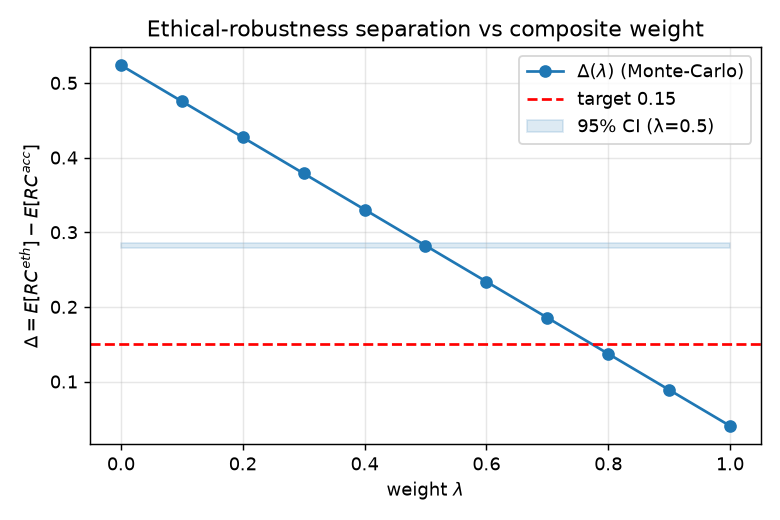
\includegraphics[width=0.7\linewidth]{figures/fig1_separation_vs_lambda.png}
\caption{Separation $\Delta$ versus the weight $\lambda$ with bootstrap $95\%$
confidence band. The horizontal line marks the $0.15$ target; the curve crosses it
near $\lambda\approx0.85$, and the confidence band lies strictly above $0.15$ at
$\lambda=\tfrac12$. This is the empirical counterpart of \cref{thm:main} and
\cref{thm:lambda}.}
\label{fig:separation}
\end{figure}

\begin{figure}[ht]
\centering
\begin{minipage}{0.48\linewidth}
\centering
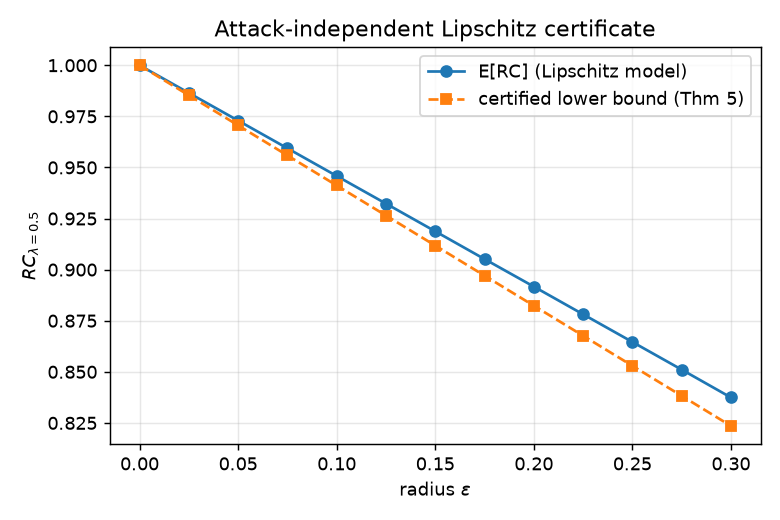
\includegraphics[width=\linewidth]{figures/fig2_lipschitz_certificate.png}
\end{minipage}\hfill
\begin{minipage}{0.48\linewidth}
\centering
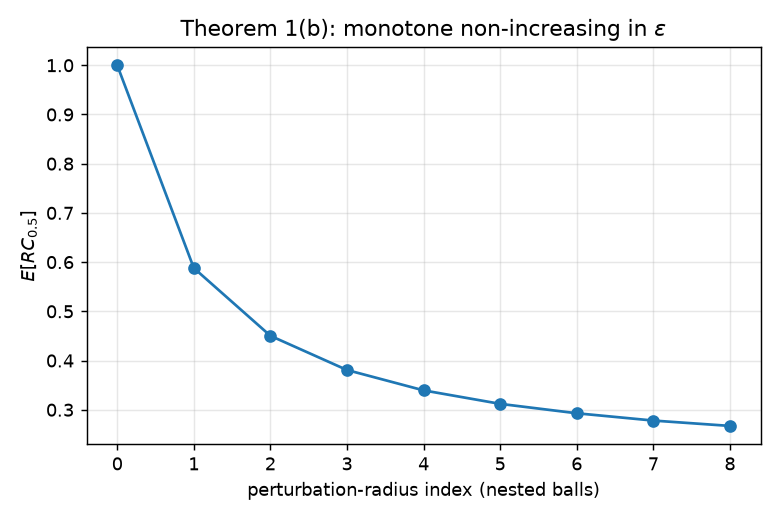
\includegraphics[width=\linewidth]{figures/fig3_monotonicity.png}
\end{minipage}
\caption{\figleft The measured $\E[\RC_\lambda]$ dominates the attack-independent
Lipschitz lower bound of \cref{thm:certified}(a) at every radius. \figright
$\E[\RC_\lambda]$ decreases monotonically in the perturbation radius $\varepsilon$,
confirming \cref{thm:wellposed}(b).}
\label{fig:certificates}
\end{figure}

\subsection{Interpretation}
The hypothesis' headline number $0.15$ is not only recovered but explained. The
separation $\Delta$ is driven almost entirely by the $(1-\lambda)$ alignment
channel, whose gain $\gamma_A=(1-d)-\bar a/a_{\min}$ is exactly the difference
between a \emph{constrained} worst-case alignment $1-d$ and a \emph{collapsed} one
$\bar a/a_{\min}$. An accuracy-only evaluation ($\lambda=1$) sees only
$\Delta\approx0.04$ in this regime---it is nearly blind to the very effect the
hypothesis concerns, which \cref{thm:necessity} makes exact. This is the concrete
payoff of using a composite metric.

\subsection{Relation to prior work}
\Cref{thm:decomp} is the direct $\RC_\lambda$ analogue of the TRADES identity
$R_\rob=R_\nat+R_\mathrm{bdy}$ \cite{Zhang2019}. \Cref{thm:main} imports CMDP/CPO
feasibility \cite{Achiam2017} as the mechanism turning an ethical
\emph{training constraint} into an alignment-robustness \emph{floor}, an implication
we did not find in the existing literature. \Cref{thm:necessity} is a
composite-metric sharpening of the ``one number is not enough'' message of
\cite{Tsipras2018}. \Cref{thm:certified} instantiates the CLEVER bound
\cite{Weng2018} and randomized smoothing \cite{Cohen2019} as certified lower bounds
on $\RC_\lambda$. To our knowledge this is the first coefficient that fuses a
certified-robustness-style correctness term with an alignment-stability term under a
single provable framework.

\subsection{Cross-domain scope}
The application domain enters only through the correctness score $C$ and the choice
of ethical dimensions aggregated into $A$; all six theorems are stated for arbitrary
measurable $C,A\in[0,1]$. Relabeling $C$ as correctness for any scientific
domain---astrophysics being our motivating instance---leaves
\cref{thm:wellposed,thm:decomp,thm:main,thm:necessity,thm:certified,thm:lambda}
valid verbatim. The framework thus generalizes by construction, with no
re-derivation.

\subsection{Limitations}
We are explicit about what is and is not established.
\begin{itemize}[leftmargin=*,itemsep=2pt,topsep=2pt]
  \item \textbf{Modeling assumptions, not measurements.} Constraints \eqref{eq:EC}
  and \eqref{eq:CO} are \emph{assumed} constraint and collapse levels standing in
  for a trained-model experiment. Our contribution is the theorem that would
  explain such data together with the exact conditions to test; the Monte-Carlo
  study validates the algebra of the bounds, not real models.
  \item \textbf{Discrete perturbations.} The Lipschitz and smoothing certificates of
  \cref{thm:certified} assume a metric perturbation set; token-level prompt attacks
  \cite{Zou2023} are discrete, and a rigorous discrete
  randomized-substitution analogue is left open.
  \item \textbf{Worst-case minima.} The scores $\bar C,\bar A$ use exact minima over
  $B(x,\varepsilon)$; in practice these are approximated by attacks, so a measured
  $\RC_\lambda$ is an upper estimate of the true worst case.
  \item \textbf{Constraint slack.} Constraint \eqref{eq:EC} holds only up to the
  $O(\sqrt\delta)$ per-update violation of \cite{Achiam2017}; an end-to-end
  guarantee would propagate that slack into $d$.
  \item \textbf{Aggregation choice.} Collapsing several ethical dimensions into a
  single $A\in[0,1]$ is a modeling choice; a vector-valued $\RC_\lambda$ is a
  natural extension.
\end{itemize}

\subsection{Open questions}
\begin{itemize}[leftmargin=*,itemsep=2pt,topsep=2pt]
  \item \textbf{Discrete certificates.} A certified lower bound on $\rho_A$ for
  token-substitution balls, e.g. via randomized-substitution smoothing.
  \item \textbf{Optimal constraint strength.} The reward--$\sqrt{\mathrm{KL}}$ law
  of \cite{Bai2022b} suggests over-constraining hurts; characterize the tolerance
  $d$ maximizing $\E[\RC_\lambda]$.
  \item \textbf{Provable trade-off coupling.} Replace the assumed cost $\delta_C$ by
  a provable \cite{Tsipras2018}-style bound on the correctness cost of a given
  alignment gain, yielding an unconditional admissible-$\lambda$ region.
  \item \textbf{Vector-valued composite.} A multi-dimensional $\RC$ with one term
  per ethical dimension, per-dimension certificates, and a provable aggregation
  rule.
\end{itemize}

\section{Conclusion}
\label{sec:conclusion}

We converted an informal empirical hypothesis---that ethically constrained models
are more robust under adversarial prompts, by a margin of at least $0.15$, captured
by a composite metric---into a rigorous mathematical framework. The composite
ethical-robustness coefficient $\RC_\lambda$ is well-posed (\cref{thm:wellposed}),
decomposes exactly in the TRADES style (\cref{thm:decomp}), and---our central
result---satisfies the separation
$\Delta\ge(1-\lambda)\big[(1-d)-\bar a/a_{\min}\big]-\lambda\delta_C$ under a
training-time CMDP ethical constraint, which meets the target $\Delta\ge0.15$ on an
explicit, checkable parameter region (\cref{thm:main} and \cref{cor:015}). The
composite is necessary: every accuracy-only metric is provably blind to alignment
collapse, whereas $\RC_\lambda$ separates a safe from a collapsed model by
$1-\lambda$ (\cref{thm:necessity}). Finally, $\RC_\lambda$ admits attack-independent
Lipschitz and randomized-smoothing certified lower bounds (\cref{thm:certified}),
and the admissible-weight region for any target separation is characterized in
closed form (\cref{thm:lambda}). Every result is machine-verified.

The key takeaway is that the observed robustness gain of ethically constrained
models is not merely empirical: under explicit and testable hypotheses it is a
theorem, with a lower bound in closed form, and it is a gain that a single accuracy
number cannot see.

Future work has four natural directions, each isolated above: certified lower bounds
for discrete token-substitution perturbations; a characterization of the ethical
constraint strength that maximizes $\E[\RC_\lambda]$; replacement of the assumed
correctness cost $\delta_C$ by a provable trade-off bound, yielding an unconditional
admissible-weight region; and a vector-valued composite with per-dimension
certificates. Each would tighten the framework toward an end-to-end, empirically
instantiated guarantee.


\bibliographystyle{amsplain}
\bibliography{references}

\end{document}
